\documentclass[12pt, letter]{article}

\usepackage{pgfplots, pgfplotstable}
\usepackage{amsmath}

\makeatletter
\long\def\ifnodedefined#1#2#3{%
    \@ifundefined{pgf@sh@ns@#1}{#3}{#2}%
}

\pgfplotsset{
    discontinuous/.style={
    scatter,
    scatter/@pre marker code/.code={
        \ifnodedefined{marker}{
            \pgfpointdiff{\pgfpointanchor{marker}{center}}%
             {\pgfpoint{0}{0}}%
             \ifdim\pgf@y>0pt
                \tikzset{options/.style={mark=*}}
                \draw [densely dashed] (marker-|0,0) -- (0,0);
                \draw plot [mark=*, mark options={fill=white}] coordinates {(marker-|0,0)};
             \else
                \tikzset{options/.style={mark=none}}
             \fi
        }{
            \tikzset{options/.style={mark=none}}        
        }
        \coordinate (marker) at (0,0);
        \begin{scope}[options]
    },
    scatter/@post marker code/.code={\end{scope}}
    }
}
\makeatother

\title{Homework 5}
\author{Martin Mueller}
\date{Due: March $4^{th}$, 2019}

\begin{document}
\maketitle

\begin{center}
	\underline{\textbf{Chapter 3}}
\end{center}

\textbf{4. A discrete random variable $X$ has the following pmf:}
$$p(x) = k(8 – x)\text{ for }x = 0,1,2,3,4,5$$

\qquad \textbf{a) Find the constant $k$.}
\begin{center}
	First, let's begin by finding out each probability in terms of $k$ for each $x$ value:
	\begin{align*}
		x = 0&: p(0) = k(8 - (0)) = 8k \\
		x = 1&: p(1) = k(8 - (1)) = 7k \\
		x = 2&: p(2) = k(8 - (2)) = 6k \\
		x = 3&: p(3) = k(8 - (3)) = 5k \\
		x = 4&: p(4) = k(8 - (4)) = 4k \\
		x = 5&: p(5) = k(8 - (5)) = 3k
	\end{align*}
	Now from one of the probability axioms, we know that the sum of all the probabilities in a given sample space must be equal to 1. Therefore:
	$$8k + 7k + 6k + 5k + 4k + 3k = 1$$
	Now we just solve for $k$:
	\begin{align*}
		33k &= 1 \\
		k &= \boxed{\frac{1}{33}}
	\end{align*}
\end{center}

\pagebreak

\qquad \textbf{b) Find the cdf of $X$ and graph it.}
\begin{center}
	First, we need to determine each probability for each $x$:
	\begin{align*}
		p(0) = 8k = \frac{8}{33} \\
		p(1) = 7k = \frac{7}{33} \\
		p(2) = 6k = \frac{6}{33} \\
		p(3) = 5k = \frac{5}{33} \\
		p(4) = 4k = \frac{4}{33} \\
		p(5) = 3k = \frac{2}{33}
	\end{align*}
	In order to construct a cdf from a pmf, we simply need to determine the proper intervals over which each given $p(x)$ value is valid, and we need to sum up each probability every time a new interval needs to be specified. For example: any $x$ value less than 0 has no chance of happening, while an $x$ value of 1 would also need to take into the account the probability of $x$ being less than 1.
	\def\arraystretch{1.2}
	\[
    F(x) = \left\{\begin{array}{cc}
        0 & x < 0 \\
        \frac{8}{33} & 0 \le x < 1 \\
        \frac{15}{33} & 1 \le x < 2 \\
        \frac{21}{33} & 2 \le x < 3 \\
        \frac{26}{33} & 3 \le x < 4 \\
        \frac{30}{33} & 4 \le x < 5 \\
        1 & x \ge 5 
        \end{array}\right.
	\]
\end{center}

\pagebreak

{\centering
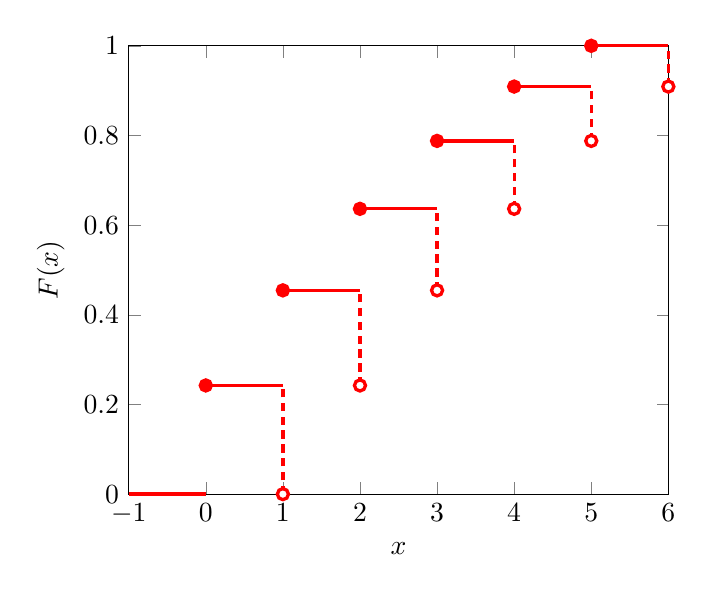
\begin{tikzpicture}
\begin{axis}[
	xlabel=$x$,
	ylabel=$F(x)$,
    clip=false,
    jump mark left,
    ymin=0,ymax=1,
    xmin=-1, xmax=6,
    every axis plot/.style={very thick},
    discontinuous,
    table/create on use/cumulative distribution/.style={
        create col/expr={\pgfmathaccuma + \thisrow{f(x)}}   
    }
]
\addplot [red] table [y=cumulative distribution]{
x f(x)
-1 0
0 8/33
1 7/33
2 6/33
3 5/33
4 4/33
5 3/33
6 0
};
\end{axis}
\end{tikzpicture}
\par}

\qquad \textbf{c) Compute $E(X)$ and $V(X)$.}
$$E(X)=\left(0 \cdot \frac{8}{33}\right)+\left(1 \cdot \frac{7}{33}\right)+\left(2 \cdot \frac{6}{33}\right)+\left(3 \cdot \frac{5}{33}\right)+\left(4 \cdot \frac{4}{33}\right)+\left(5 \cdot \frac{3}{33}\right)=\boxed{1.9697}$$
\begin{multline*}
	V(X)=E(X^{2})-[E(X)]^{2}= \\
	\left(0^{2} \cdot \frac{8}{33}\right)+\left(1^{2} \cdot \frac{7}{33}\right)+\left(2^{2} \cdot \frac{6}{33}\right) \\
	+\left(3^{2} \cdot \frac{5}{33}\right)+\left(4^{2} \cdot \frac{4}{33}\right)+\left(5^{2} \cdot \frac{3}{33}\right) \\
	-(1.9697)^{2}=\boxed{2.6354}
\end{multline*}

\qquad \textbf{d) Find $E(3X - 5)$ and $V(3X - 5)$.}
$$E(3X-5)=3E(X)-5=3(1.9697)-5=\boxed{0.9091}$$
$$V(3X-5)=3^{2}V(X)=9 \cdot 2.6354=\boxed{23.7186}$$


\textbf{6. A box contains two \$20 bills, three \$10 bills, and one \$5 bill. You remove bills one at a time at random from the box until you remove a \$10 bill.}

\pagebreak

\qquad \textbf{a) If $X$ is the random variable that represents the total number of bills removed from the box, find the mean, variance, and standard deviation of $X$.}
\begin{center}
	For this particular problem, we only care about drawing a \$10 bill. Because of that, we'll group the bills into 2 categories: \$10 bills (of which there are 3) and non-\$10 bills (of which there are also 3). The probability of getting a \$10 bill on the first go is the number of \$10 bills divided by the total number of bills which is $\frac{3}{6}$ or $\frac{1}{2}$. The probability of getting a \$10 on the next go is $\frac{3}{6} \cdot \frac{3}{5}$ or $\frac{3}{10}$. This goes on until 3 bills have been drawn. After that point, it is guaranteed that a \$10 bill will be drawn, (this puts the stopping point of the pmf at 4 bills). From this data, we can create a pmf (\underline{Note:} I adjusted the fractions to all have a common denominator):
	\linebreak
	\linebreak
	\def\arraystretch{1.5}
	\begin{tabular}{|c|c|c|c|c|c|c|}
		\hline
		$X$ & 1 & 2 & 3 & 4 \\
		\hline
		$p(x)$ & $\frac{10}{20}$ & $\frac{6}{20}$ & $\frac{3}{20}$ & $\frac{1}{20}$ \\
		\hline
	\end{tabular}
	\linebreak
	\linebreak
	Now we just plug these values into the formulas to calculate the figures we want:
	$$E(X)=\left(1 \cdot \frac{10}{20}\right)+\left(2 \cdot \frac{6}{20}\right)+\left(3 \cdot \frac{3}{20}\right)+\left(4 \cdot \frac{1}{20}\right)=\boxed{1.75}$$
	\begin{multline*}
		V(X)=E(X^{2})-[E(X)]^{2}= \\
		\left(1^{2} \cdot \frac{10}{20}\right)+\left(2^{2} \cdot \frac{6}{20}\right)+\left(3^{2} \cdot \frac{3}{20}\right) \\
		+\left(4^{2} \cdot \frac{1}{20}\right)-(1.75)^{2}=\boxed{1.2375}
	\end{multline*}
	$$\sigma_{x}=\sqrt{V(X)}=\boxed{1.1124}$$
\end{center}

\pagebreak

\qquad \textbf{b) If $Y$ is the random variable that represents the total value of bills removed from the box, find the mean, variance, and standard deviation of $Y$.}
\begin{center}
	Just as in part a, only 4 bills maximum will be drawn from the box. This means that the maximum value of those 4 bills would be \$55 (if 2 \$20 bills, 1 \$5 bill, and 1 \$10 bill were drawn). The minimum value of the cash drawn would be \$10 (if a \$10 were drawn immediately). Now that we have our range, we just have to figure out how many different combinations there would be for each scenario. By doing so, we can construct the following pmf (\underline{Note:} I adjusted the fractions to all have a common denominator):
	\linebreak
	\linebreak
	\def\arraystretch{1.5}
	\begin{tabular}{|c|c|c|c|c|c|c|}
		\hline
		$Y$ & \$10 & \$15 & \$30 & \$35 & \$50 & \$55 \\
		\hline
		$p(y)$ & $\frac{20}{40}$ & $\frac{6}{40}$ & $\frac{6}{40}$ & $\frac{3}{40}$ & $\frac{3}{40}$ & $\frac{2}{40}$ \\
		\hline
	\end{tabular}
	\linebreak
	\linebreak
	Now we just plug these values into the formulas to calculate the figures we want:
	\begin{multline*}
	E(Y)=\left(\$10 \cdot \frac{20}{40}\right)+\left(\$15 \cdot \frac{6}{40}\right)+\left(\$30 \cdot \frac{6}{40}\right)+\left(\$35 \cdot \frac{3}{40}\right) \\
	+\left(\$50 \cdot \frac{3}{40}\right)+\left(\$55 \cdot \frac{2}{40}\right)=\boxed{\$20.875}
	\end{multline*}
	\begin{multline*}
		V(Y)=E(Y^{2})-[E(Y)]^{2}= \\
		\left(\$10^{2} \cdot \frac{20}{40}\right)+\left(\$15^{2} \cdot \frac{6}{40}\right)+\left(\$30^{2} \cdot \frac{6}{40}\right)+\left(\$35^{2} \cdot \frac{3}{40}\right) \\
	+\left(\$50^{2} \cdot \frac{3}{40}\right)+\left(\$55^{2} \cdot \frac{2}{40}\right)-(\$20.875)^{2}=\boxed{213.6094}
	\end{multline*}
	$$\sigma_{y}=\sqrt{V(Y)}=\boxed{\$14.6154}$$
\end{center}

\textbf{12. A book shop owner orders copies of a certain magazine for its magazine rack 
each week. The shop owner pays \$4 for each copy of the magazine and sells it at \$6. Let $X$ = demand for the magazine, with pmf:}
\begin{center}
	\begin{tabular}{|c|c|c|c|c|c|c|}
		\hline
		$X$ & 1 & 2 & 3 & 4 & 5 & 6 \\
		\hline
		$p(x)$ & .08 & .16 & .22 & .30 & .18 & .06 \\
		\hline
	\end{tabular}
\end{center}

\pagebreak

\textbf{a) Determine the optimal number of magazines the shop owner should order to maximize the profit.}
\begin{center}
	In order to determine the optimal number of magazines to buy, we must first compute pmfs that compare potential net gain to probability for the shop owner buying 1, 2, 3, 4, 5, or 6 magazines:
	\linebreak
	\linebreak
	\begin{tabular}{|c|c|c|c|c|c|c|}
		\hline
		1 magazine & \$2 & \$2 & \$2 & \$2 & \$2 & \$2 \\
		\hline
		2 magazines & -\$2 & \$4 & \$4 & \$4 & \$4 & \$4 \\
		\hline
		3 magazines & -\$6 & \$0 & \$6 & \$6 & \$6 & \$6 \\
		\hline
		4 magazines & -\$10 & -\$4 & \$2 & \$8 & \$8 & \$8 \\
		\hline
		5 magazines & -\$14 & -\$8 & -\$2 & \$4 & \$10 & \$10 \\
		\hline
		6 magazines & -\$18 & -\$12 & -\$6 & \$0 & \$6 & \$12 \\
		\hline
		Probability & .08 & .16 & .22 & .30 & .18 & .06 \\
		\hline
	\end{tabular}
	\linebreak
	\linebreak
	After that, we have to calculate the expected values for each of the pmfs:
	\begin{multline*}
		E(\text{1 magazine})=\left(\$2 \times .08\right)+\left(\$2 \times .16\right)+\left(\$2 \times .22\right) \\
		+\left(\$2 \times .30\right)+\left(\$2 \times .18\right)+\left(\$2 \times .06\right)=\$2.00
	\end{multline*}
	\begin{multline*}
		E(\text{2 magazines})=\left(-\$2 \times .08\right)+\left(\$4 \times .16\right)+\left(\$4 \times .22\right) \\
		+\left(\$4 \times .30\right)+\left(\$4 \times .18\right)+\left(\$4 \times .06\right)=\$2.08
	\end{multline*}
	\begin{multline*}
		E(\text{3 magazines})=\left(-\$6 \times .08\right)+\left(\$0 \times .16\right)+\left(\$6 \times .22\right) \\
		+\left(\$6 \times .30\right)+\left(\$6 \times .18\right)+\left(\$6 \times .06\right)=\$4.08
	\end{multline*}
	\begin{multline*}
		E(\text{4 magazines})=\left(-\$10 \times .08\right)+\left(-\$4 \times .16\right)+\left(\$2 \times .22\right) \\
		+\left(\$8 \times .30\right)+\left(\$8 \times .18\right)+\left(\$8 \times .06\right)=\$3.32
	\end{multline*}
	\begin{multline*}
		E(\text{5 magazines})=\left(-\$14 \times .08\right)+\left(-\$8 \times .16\right)+\left(-\$2 \times .22\right) \\
		+\left(\$4 \times .30\right)+\left(\$10 \times .18\right)+\left(\$10 \times .06\right)=\$0.76
	\end{multline*}
	\begin{multline*}
		E(\text{6 magazines})=\left(-\$18 \times .08\right)+\left(-\$12 \times .16\right)+\left(-\$6 \times .22\right) \\
		+\left(\$0 \times .30\right)+\left(\$6 \times .18\right)+\left(\$12 \times .06\right)=-\$2.88
	\end{multline*}
	Lastly, we simply compare the expected values, determine which one is highest, and figure out the optimal number of magazines to purchase based on our statistical analysis. Since 3 magazines yielded the highest expected profit, we can conclude that it would be the wisest decision to purchase $\boxed{\text{3 magazines}}$ in order to maximize profit.
\end{center}

\textbf{b) What is the expected maximum profit?}
\begin{center}
	\textit{See p. 6 for work.} $\boxed{\$4.08}$
\end{center}
\end{document}